\documentclass[11pt]{article}
\usepackage{amsmath}
\usepackage{xeCJK}
\usepackage{amsfonts}
\usepackage{color}
\usepackage[hidelinks]{hyperref}
\usepackage{listings}
\usepackage{graphicx}
\usepackage{multirow}
\usepackage{algorithm,algpseudocode}

\title{Support Vector Machine}
\author{Wenfeng Luo, 18214551}
\date{}
\begin{document}
\maketitle
本文讨论支持向量机(Support Vector Machine)分类器中涉及的二次规划问题。章节\ref{notation}列出本文用到的符号表示;章节\ref{formulation}形式化定义支持向量机分类器涉及的优化问题,包括线性可分以及不可分两种情形;章节\ref{duality}讨论如何通过拉格朗日对偶性得到等价的仅关于拉格朗日乘子的对偶优化问题;章节\ref{optimization}介绍两种优化算法用于求解相关的对偶问题,分别是简化版的序列最小化算法(Sequential Minimal Optimization)和基于二阶梯度信息的改进版本;章节\ref{implementation}简单介绍实现细节;章节\ref{experiment}给出了上述优化算法的实验结果,并比较两种优化算法的运行效率。
\section{Notation}\label{notation}
在深入讨论之前,先声明本文用到的一些符号规定:
\begin{itemize}
\item 训练数据:$\{(x^{(1)}, y^{(1)}), ..., (x^{(m)}, y^{(m)})\}, x^{(i)}\in R^n, y^{(i)}\in\{1, -1\}$
\item 模型参数:$w, b$
\item 分类器:$h_{w, b}(x)=g(w^Tx+b)$。 如果$g(z) > 0$,预测为1,否则预测为-1。
\end{itemize}

\section{Problem Formulation}\label{formulation}
\subsection{Linearly Separable}
当我们的数据集线性可分时(如图\ref{img1}),我们希望得到这样一个决策边界$P_0$,它到最近的正样本和负样本的距离是最远的。我们可以形式化为对应边界的两条直线$P_1$和$P_2$之间的距离最大。容易知道两直线的距离为:
\begin{equation}
\text{margin} = \frac{k - (-k)}{\sqrt{w_1^2+...+w_n^2}} = \frac{2k}{||w||_2}
\end{equation}
\begin{figure}
	\centering
	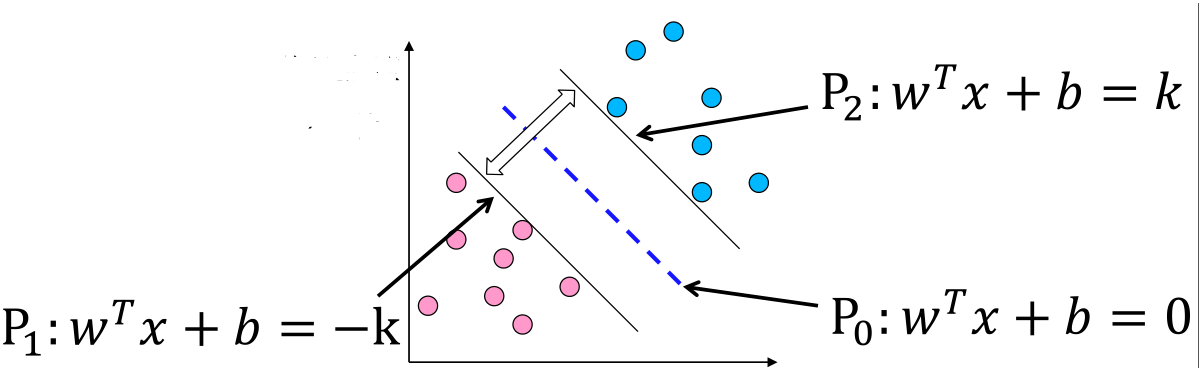
\includegraphics[height=4cm]{images/img4.png}
	\caption{最大间隔分类器}
	\label{img1}
\end{figure}
于是我们可以得到第一个优化问题
\begin{align}
\begin{split}
\max_{w, b, k}\quad&\frac{2k}{||w||_2}\\
\text{s.t.}\quad&w^Tx^{(i)}+b>=k\text{ for }y^{(i)}=1\\
&w^Tx^{(i)}+b<=-k\text{ for }y^{(i)}=-1\\
&k>0
\end{split}
\end{align}
简化一下,可以把正负训练样本的约束条件写成统一的式子
\begin{align}
\begin{split}
\max_{w, b, k}\quad&\frac{2k}{||w||_2}\\
\text{s.t.}\quad&y^{(i)}(w^Tx^{(i)}+b)>=k\quad i = 1,...,m\\
&k>0
\end{split}
\end{align}
通过简单的变量替换(取$w'=\frac{w}{k}, b'=\frac{b}{k}$),我们可以发现$k$是无关紧要的。另外,我们还可再变换一下形式,因为优化某个函数的最大值等价优化该函数的倒数的最小值,并且这样做以后方便我们对参数$w$的求导。于是可以得到如下的等价优化问题
\begin{align}\label{eq:2}
\begin{split}
\min_{w, b}\quad&\frac{1}{2}w^Tw\\
\text{s.t.}\quad&y^{(i)}(w^Tx^{(i)}+b)>=1\quad i = 1,...,m\\
\end{split}
\end{align}
\subsection{Linearly Non-separable and Regularization}
上述的讨论只适用于数据集线性可分的情况,但很多时候我们不能找到一条直线将数据集完美地划分正负样本,如图\ref{img2}(a)。此外,有些时候我们也不期望分分类器完美地划分训练集,比如训练集有部分离群点的情形,这些离群点对决策边界起极大的扰动作用,如图\ref{img2}(b)。所以,我们可以考虑让某些点的约束条件不严格成立,同时对不成立的约束条件引入某种惩罚项,比如$l_1$正则,于是可以在原来的基础上得到新的优化问题
\begin{align}\label{eq:3}
\begin{split}
\min_{w, b, \xi}\quad&\frac{1}{2}w^Tw +C\sum_{i=1}^m\xi_i\\
\text{s.t.}\quad&y^{(i)}(w^Tx^{(i)}+b)>=1-\xi_i\quad i = 1,...,m\\
&\xi_i\geq 0\quad i=1,...,m
\end{split}
\end{align}
其中,$C$是一个预定义好的大于0的常数,它决定了前后两项损失的权重,类似于线性规划的正则参数。很明显,优化问题(\ref{eq:3})是一个典型的二次规划问题,我们已经可以用一般的商用包求解该问题,但是在训练样本比较大的时候求解效率是比较低下的。接下来我们考虑如何得到该问题的对偶问题,然后再讨论一个求解该对偶问题的高效迭代算法。
\begin{figure}
\centering
\begin{tabular}{cc}
	
	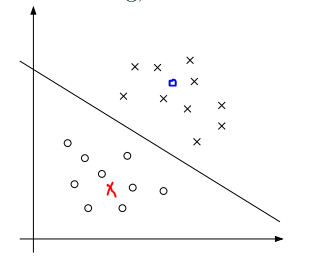
\includegraphics[width=4cm]{images/img6.png}
	& 
	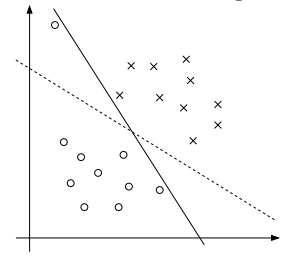
\includegraphics[width=4cm]{images/img7.png} \\
	
	(a) Linearly non-separable & (b) Outliers\\
\end{tabular}
\caption{线性不可分和离群点的情形}
\label{img2}
\end{figure}

\section{Lagrange Duality}\label{duality}
这一章节我们考虑使用拉格朗日对偶得到优化问题(\ref{eq:3})的对偶问题。先写出原问题问题的拉格朗日函数
\begin{align}
\begin{split}
L(w, b, \xi, \alpha, \beta) &= \frac{1}{2}w^Tw + C\sum_{i=1}^m\xi_i\\
&-\sum_{i=1}^m\alpha_i\left(y^{(i)}(w^Tx^{(i)} +b) - 1 + \xi_i\right) - \sum_{i=1}^m\beta_i\xi_i\\
\end{split}
\end{align}
其中,我们要求不等式约束对应的乘子$\alpha_i\geq 0, \beta_i\geq0, i=1,...,m$。分别对原问题的决策变量求导并置零,可以得到:
\begin{align}
\frac{\partial L}{\partial w}&=0\to w = \sum_{i=1}^m\alpha_iy^{(i)}x^{(i)}\\
\frac{\partial L}{\partial b}&=0\to\sum_{i=1}^m\alpha_iy^{(i)}=0\\
\frac{\partial L}{\partial \xi_i}&=0\to\beta_i= C-\alpha_i
\end{align}
从最后一个等式我们还可以得到$\alpha_i$的另外一个约束,因为$\beta_i\geq 0$,因此$0\leq \alpha_i \leq C$。利用上面的等式关系回代回拉格朗日函数,可以得到只与乘子$\alpha$有关的对偶函数:
\begin{align}
\begin{split}
g(\alpha) =\sum_{i=1}^m\alpha_i-\frac{1}{2}\sum_{i,j=1}^m\alpha_i\alpha_jy^{(i)}y^{(j)}\langle x^{(i)}, x^{(j)}\rangle
\end{split}
\end{align}
根据对偶性,原问题等价于求解如下的对偶问题
\begin{align}\label{eq:1}
\begin{split}
\max_\alpha\quad&\sum_{i=1}^m\alpha_i-\frac{1}{2}\sum_{i,j=1}^m\alpha_i\alpha_jy^{(i)}y^{(j)}\langle x^{(i)}, x^{(j)}\rangle\\
\text{s.t.}\quad&0\leq\alpha_i\leq C\quad i=1,...,m\\
&\sum_{i=1}^m\alpha_iy^{(i)}=0
\end{split}
\end{align}
为了判别算法的收敛性,我们可以列出上述问题的KKT条件
\begin{itemize}
\item $\alpha_i=0, y^{(i)}(w^Tx^{(i)}+b)\geq 1$:$x^{(i)}$在边界以外;
\item $0< \alpha< C, y^{(i)}(w^Tx^{(i)}+b) = 1$:$x^{(i)}$刚刚好在边界上面;
\item $\alpha_i=C, y^{(i)}(w^Tx^{(i)}+b) \leq 1$:$x^{(i)}$在边界以内。
\end{itemize}
这里说的边界就是图\ref{img1}中的直线$P_1$和$P_2$。上述的条件非常重要,因为在后续介绍的SMO算法就是选取那些没有满足上述条件的乘子$\alpha_i$来进行优化。
\section{SMO algorithm}\label{optimization}
优化问题(\ref{eq:2}, \ref{eq:3}, \ref{eq:1})都是二次规划问题,可以用通用的程序求解,但时间效率比较低下。下面讨论如何在有约束条件下使用坐标下降方法高效快速求解关于拉格朗日乘子的优化问题(\ref{eq:1}),求解到最优的$\alpha^*$以后,我们可以通过如下方式恢复原来的参数
\begin{align}\label{eq:wb}
\begin{split}
w=&\sum_{i=1}^m\alpha_iy^{(i)}x^{(i)}\\
b=&-\frac{1}{2}\left(\min_{y^{(i)}=1}w^Tx^{(i)} + \max_{y^{(i)}=-1}w^Tx^{(i)}\right)
\end{split}
\end{align}
4.1章节简单介绍坐标下降方法的相关知识;4.2章节讲解序列最小化算法(Sequential Minimal Optimization)的一个简单实现版本;4.3章节介绍SMO的一种改进版本,该版本使用了二阶信息去选取优化的拉格朗日乘子,比原有的简单实现更高效快速,而且能确保收敛到最优值。

\subsection{Coordinate Descent}
首先我们考虑一个无约束的优化问题
\begin{equation}
\max_\alpha\quad f(\alpha_1, \alpha_2, ..., \alpha_n)
\end{equation}
坐标下降方法每次只选取其中一个决策变量而固定其他所有的变量进行优化,这样以来我们每一次迭代需要求解的子问题就变得很简单,只是关于一个一元函数的最小化。另外,如果这个一元函数有特殊的结构,比如是关于$\alpha_i$的二次函数,那么子问题的优化是有解析解的,因此可以很容易求解。我们可以写出坐标下降方法的简单过程

\begin{algorithm}[H] 
	\caption{Coordinate Descent}
	\label{alg:loop}
	\begin{algorithmic}[1]
		\Statex
		\State{Initialize all $\alpha$'s}
		\While{Not convergent}
		\For{$i \gets 1$ to $n$}
		\State{$\alpha_i=\text{argmax}_{\hat{\alpha_i}}\quad f(\alpha_1,..., \alpha_{i-1}, \hat{\alpha_{i}}, \alpha_{i+1}, ..., \alpha_n)$}
		\EndFor
		\EndWhile
	\end{algorithmic}
\end{algorithm}

当然,我们还可以借助一些启发式的策略来决定决策变量的优化顺序,以加快算法收敛速率。

\subsection{Slow Version}
要将上述的坐标下降方法用于我们的优化问题,我们还得考虑问题(\ref{eq:1})中的等式约束。由于问题中的等式约束,我们每次优化的时候如果只选取一个乘子,那么我们没有优化的余地了。SMO算法的思想就是每次选取两个乘子进行优化,这时候我们要解决的子问题就是简单的二次函数的优化。举个例子,如果我们选取$\alpha_1, \alpha_2$为优化变量而固定其他的乘子,利用问题(\ref{eq:1})的等式约束可以得到这两个乘子之间的关系为
\begin{align}
\begin{split}
\alpha_1y^{(1)} + \alpha_2y^{(2)} &= \zeta\\
\zeta &=-\sum_{i=3}^m \alpha_iy^{(i)}
\end{split}
\end{align}
$\zeta$在优化$\alpha_1, \alpha_2$时保持不变。另外,我们还要考虑拉格朗日乘子的框式约束,图\ref{img:lh}描述了两个乘子在框式约束下的有效区域。
\begin{figure}
\centering
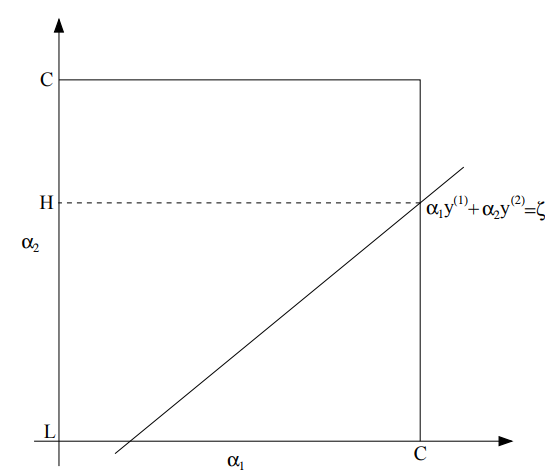
\includegraphics[width=6cm]{images/img14.png}
\caption{乘子$\alpha_1, \alpha_2$的约束条件}
\label{img:lh}
\end{figure}
利用等式关系替换$\alpha_1 = y^{(1)}(\zeta - \alpha_2y^{(2)})$,因此我们只需要考虑$\alpha_2$的约束条件以使得最优解有效。考虑不同的情形,$\alpha_2$的上下界分别为
\begin{enumerate}
\item $y^{(1)} = y^{(2)}$时,$L=\max(0, \alpha_1 + \alpha_2 - C), H=\min(C, \alpha_1+\alpha_2)$;
\item $y^{(1)} \neq y^{(2)}$时,$L=\max(0, \alpha_2-\alpha_1), H=\min(C, C+\alpha_2-\alpha_1)$。
\end{enumerate}
综上所述,我们需要在$[L, H]$区间内最优化一个关于$\alpha_2$的二次函数。另外,由点积的性质我们知道$2\langle x, y\rangle-\langle x, x\rangle - \langle y, y\rangle \leq 0$,因此这个二次函数的二次项系数是小于等于0的。记$\alpha^{uc}_2$为对称轴的位置,有如下三种情况
\setlength\tabcolsep{1.5pt}
\begin{tabular}{ccc}
	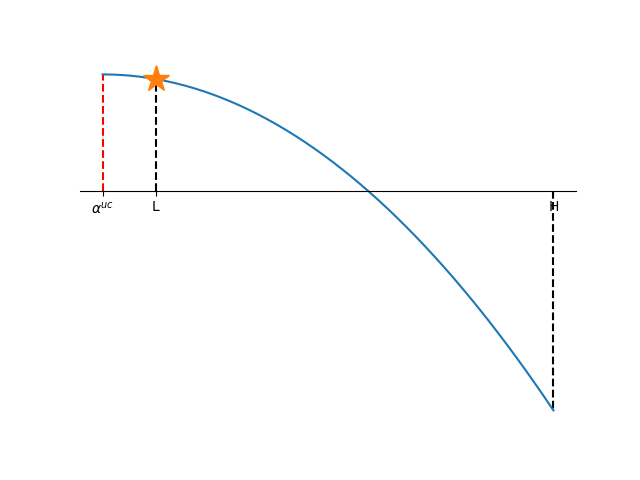
\includegraphics[width=0.33\textwidth]{images/img13.png} & 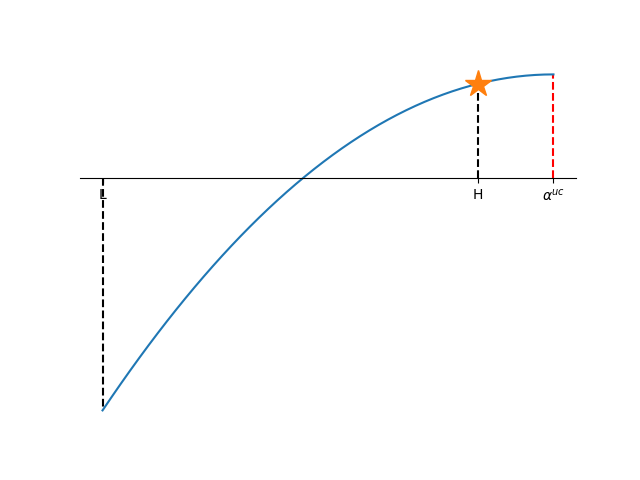
\includegraphics[width=0.33\textwidth]{images/img12.png} &
	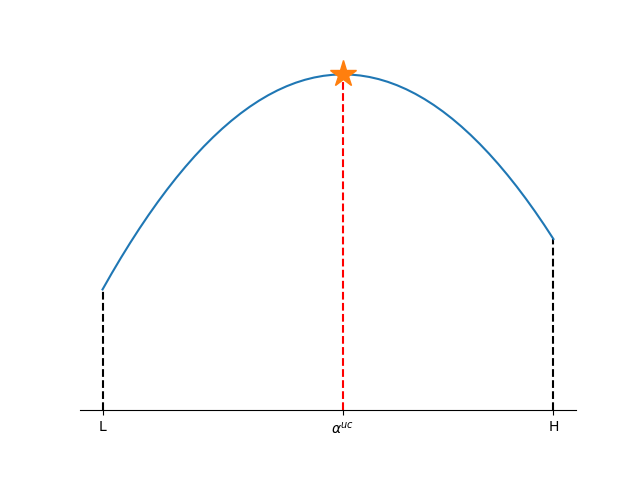
\includegraphics[width=0.33\textwidth]{images/img11.png}\\
	(1) $\alpha_2^{uc} < 0$ & (2) $\alpha_2^{uc} > C$ &
	(3) $0 \leq \alpha_2^{uc} \leq C$ 
\end{tabular}
上述三种情况可以用一个式子表示
\begin{align}
\alpha_2^* = \min(\max(L, \alpha^{uc}_2), H)
\end{align}
下面给出SMO的简单实现版本
\begin{algorithm}
	\caption{Simple Implementation of SMO}
	\label{alg:simple_smo}
	\textbf{Input:} $\{(x^{(1)}, y^{(1)}),...(x^{(m)}, y^{(m)})\}$\\
	\textbf{Output:} $w, b$
	\begin{algorithmic}[1]
		\Statex
		\State{Initialize all $\alpha$'s to 0}
		\State{tol=10, iter=0}
		\While{iter < tol}
		\State{iter = iter + 1}
		\For{$i \gets 1$ to $m$}
		\If{KKT condition not satisfied for $\alpha_i$}
		\State{Randomly choose another $\alpha_j$}
		\State{Compute the lower bound $L$ and upper bound $H$ for $\alpha_j$}
		\If{$L = H$}
		\State{\textbf{break}}
		\EndIf
		\State{iter = 0}
		\State{Compute the unclipping value $\alpha_{j}^{uc}$ for $\alpha_j$}
		\State{$\zeta = \alpha_i^{old}y^{(i)}+\alpha_j^{old}y^{(j)}$}
		\State{$\alpha_j^{new} =  \min(\max(L, \alpha^{uc}_j), H)$}
		\State{$\alpha_i^{new} =  y^{(i)}(\zeta - \alpha_j^{new}y^{(j)})$}
		\EndIf
		\EndFor
		\EndWhile
		\State{Use equation (\ref{eq:wb}) to Compute $w, b$ from $\alpha$'s}
	\end{algorithmic}
\end{algorithm}
算法\ref{alg:simple_smo}中需要指定一个超参数tol,该超参数表明当连续遍历整个数据集tol次的时候,都没有发现可以更新的乘子了,那么算法终止。当完成拉格朗日乘子的优化以后,我们通过公式\ref{eq:wb}计算模型原来的参数$w,b$。得到模型的参数以后,就可以对新的样本进行预测了。
\subsection{Fast Version}
算法\ref{alg:simple_smo}由于只是简单地随机选取第二个乘子,因此效率比较低下。这一章节介绍libsvm库中基于二阶导数信息的乘子选取方式。在讨论新的选取乘子方法之前,我们先定义一些符号:
\begin{align}
\begin{split}
a_{ij} &= K_{ii}+K_{jj} - 2K_{ij}\\
b_{ij} &= -y_i\nabla f(\alpha)_i + y_j\nabla f(\alpha)_j\\
I_{up}(\alpha) &= \{t|\alpha_t < C, y_t=1\text{ or }\alpha_t > 0, y_t=-1\}\\
I_{low}(\alpha) &= \{t|\alpha_t < C, y_t=-1\text{ or }\alpha_t > 0, y_t=1\}
\end{split}
\end{align}
上面的符号中,$K$即核矩阵,如果是简单的线性和函数,其中的元素$K_{ij}$即为$\langle x^{(i)}, x^{(j)}\rangle$。$I_{up}$和$I_{low}$表示两类不同的违背了KKT条件的乘子集合。除此之外,由于某些核函数会导致非正定的核矩阵,libsvm的实现中还对$a_{ij}$的值做了如下调整
\begin{equation}
\hat{a_{ij}} = \begin{cases}
a_{ij} & a_{ij} > 0\\
\tau & otherwise
\end{cases}
\end{equation}
$\tau$为一个非常接近于0的常量,一般取1e-12。

借鉴libsvm库的实现,在每次迭代的时候,按照如下方式选取两个乘子:
\begin{align}\label{eq:chooseij}
\begin{split}
i &= \text{argmin}_t\{y_t\nabla f(\alpha)|t\in I_{up}(\alpha)\}\\
j &= \text{argmax}_t\{-\frac{b_{ii}}{\hat{a_{it}}}|t\in I_{low},-y_t\nabla f(\alpha)_t < -y_i\nabla f(\alpha)_i\}
\end{split}
\end{align}
基于上面的讨论,我们可以给出如下新的优化算法
\begin{algorithm} 
	\caption{Improved Implementation of SMO}
	\label{alg:complete_smo}
	\textbf{Input:} $\{(x^{(1)}, y^{(1)}),...(x^{(m)}, y^{(m)})\}$\\
	\textbf{Output:} $w, b$
	\begin{algorithmic}[1]
		\Statex
		\State{Initialize all $\alpha$'s to 0}
		\State{tol=10, iter=0}
		\While{True}
		\State{Choose two multipliers $\alpha_i, \alpha_j$ using equation \ref{eq:chooseij}}
		\If{no such $\alpha_i, \alpha_j$ exist}
		\State{\textbf{break}}
		\EndIf
		\State{Compute the lower bound $L$ and upper bound $H$ for $\alpha_j$}
		\State{Compute the unclipping value $\alpha_{j}^{uc}$ for $\alpha_j$}
		\State{$\zeta = \alpha_i^{old}y^{(i)}+\alpha_j^{old}y^{(j)}$}
		\State{$\alpha_j^{new} =  \min(\max(L, \alpha^{uc}_j), H)$}
		\State{$\alpha_i^{new} =  y^{(i)}(\zeta - \alpha_j^{new}y^{(j)})$}
		\EndWhile
		\State{Use equation (\ref{eq:wb}) to Compute $w, b$ from $\alpha$'s}
	\end{algorithmic}
\end{algorithm}
\section{Implementation}\label{implementation}
代码实现在附件中,也可以在github\footnote{\url{https://github.com/irlyue/MLAlg}}上查看。主要是两个文件:
\begin{itemize}
\item \href{https://github.com/Irlyue/MLAlg/blob/master/code/svm/svm.py}{svm.py}: 该模块实现了常见的核函数,包括线性核,多项式核以及高斯核;以及一个SVM类提供训练和测试接口。
\item\href{https://github.com/Irlyue/MLAlg/blob/master/code/svm/svm_solver.py}{svm\_solver.py}: 这个模块主要实现了本文提到的两种优化算法,WSS1Solver和WSS3Solver。
\item\href{https://github.com/Irlyue/MLAlg/blob/master/notebook/svm/SVM\%20Solver\%20Comparison.ipynb}{SVM Solver Comparison.ipynb}: 涉及实验的代码。
\end{itemize}
\section{Experimental Results}\label{experiment}
\textbf{数据集 }实验使用了两个人造数据集,他们的详细描述如下:
\begin{enumerate}
	\item 数据集A: 线性可分的二分类数据,训练样本个数100,实验时统一使用线性核函数;
	\item 数据集B: 线性不可分的二分类数据,训练样本个数500,实验时统一使用高斯核函数。
\end{enumerate}
图(\ref{data})给出了两个数据的可视化结果。
\begin{figure}
	\centering
	\setlength{\tabcolsep}{0.05\textwidth}
	\begin{tabular}{cc}
		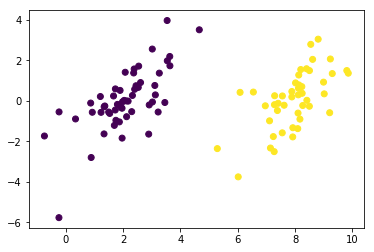
\includegraphics[width=0.4\textwidth]{images/img15.png} & 
		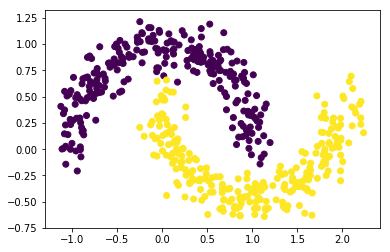
\includegraphics[width=0.4\textwidth]{images/img17.png}\\
		(a)数据集A & (b)数据集B 
	\end{tabular}
	\caption{二分类数据集}
	\label{data}
\end{figure}

\textbf{简单的二分类问题 }图(\ref{exp:1})给出了训练线性核函数的SVM在一个二分类数据集上的结果,正则参数$C=1$。
\begin{figure}
\centering
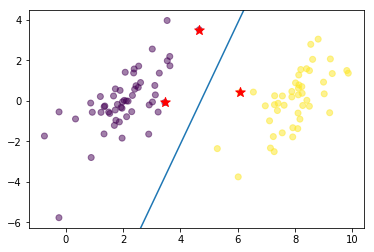
\includegraphics[width=0.5\textwidth]{images/img16.png}
\caption{线性SVM的决策边界(蓝线)以及支持向量(红)}
\label{exp:1}
\end{figure}

\textbf{两种优化算法的运行效率比较 }在这次实验中,我们比较两种算法在不同规模数据集下的性能。实验结果如表格(\ref{exp:2})所示。可以看到,算法3的运行效率要远远优于算法2。
\begin{table}
\caption{两种算法在不同规模数据集下的性能}
\label{exp:2}
\centering
\begin{tabular}{c|cc|cc}
\hline
\multirow{2}{4em}{优化算法} & \multicolumn{2}{c|}{数据集A} & \multicolumn{2}{c}{数据集B} \\ 
& 运行时间 & 支持向量的个数 & 运行时间 & 支持向量的个数  \\ 
\hline
算法2 & 103ms & 5 & 5.24s &207\\
算法3 & 5.9ms & 3 & 21.3ms & 207\\
\hline
\end{tabular}
\end{table}
\pagebreak
\section{References}
\begin{enumerate}
\item\href{http://202.116.81.74/cache/1/03/cs229.stanford.edu/f92d1f9eccf4dde766e9eba3f8231233/cs229-notes3.pdf}{CS229 Lecture notes: Support Vector Machines}
\item Fast Training of Support Vector Machines using Sequential Minimal Optimization
\item\href{http://www.jmlr.org/papers/volume6/fan05a/fan05a.pdf}{Working Set Selection Using Second Order Information for Training Support Vector Machines}
\item\href{http://www2.ift.ulaval.ca/~chaib/IFT-4102-7025/public_html/Fichiers/Machine_Learning_in_Action.pdf}{Machine Learning in Action, chapter 6}
\end{enumerate}
\end{document}